\textbf{Name:} \\

\medskip

\textbf{Conspirators:} 

\medskip
\medskip

\hrule

\medskip


%% \assignmentsonly{\pleasesubmitprojectdraft}

%% data for scaling from bettencourt

\begin{enumerate}

\item

  Use a back-of-an-envelope scaling argument to
  show that maximal rowing speed $V$ increases 
  as the number of oarspeople $N$ as $V \propto N^{1/9}$.

  Assume the following:
  \begin{enumerate}
  \item
    Rowing shells are geometrically similar (isometric).
    The table below taken from McMahon and Bonner~\cite{mcmahon1983a} shows that
    shell width is roughly proportional to shell length $\ell$.
    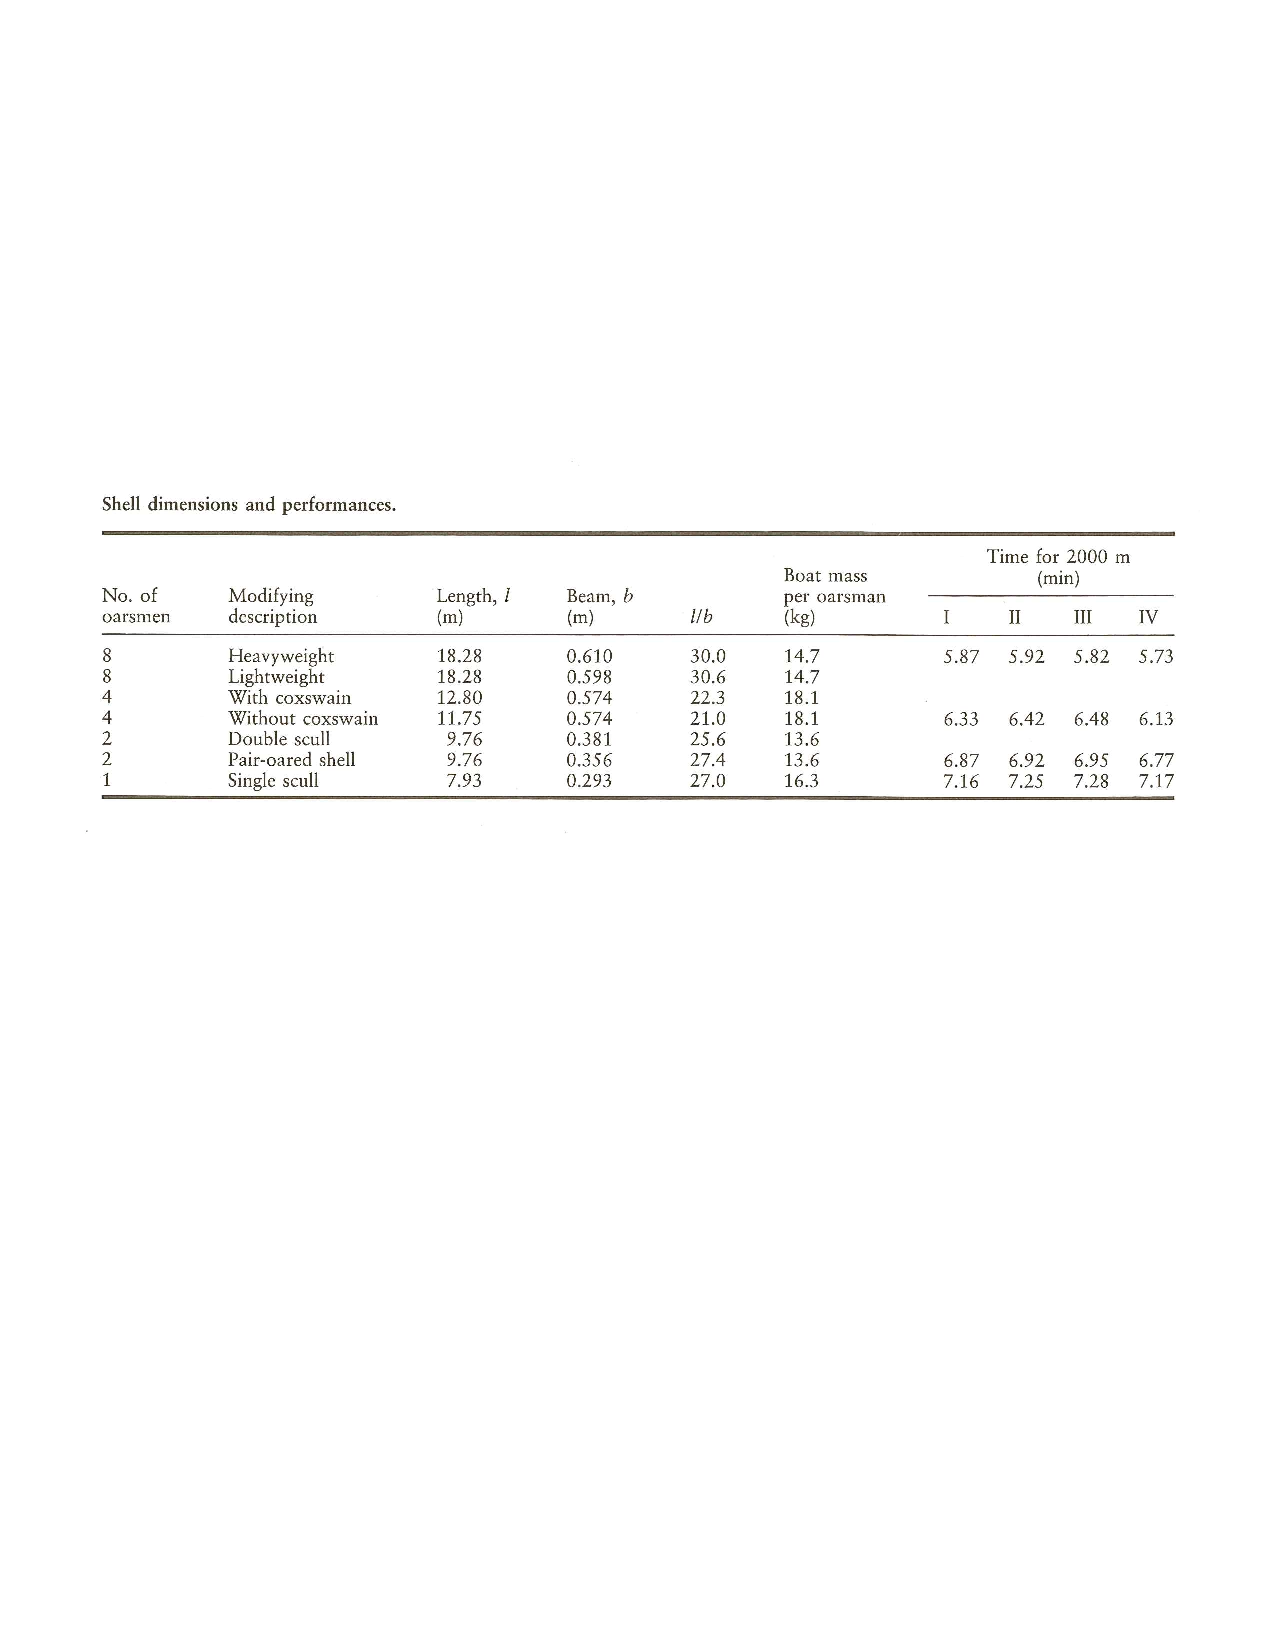
\includegraphics[width=\textwidth]{mcmahon1983a_p46rowing.pdf}
  \item
    The resistance encountered by a shell is due largely to 
    drag on its wetted surface.
  \item
    Drag force is proportional to the product of the square
    of the shell's speed ($V^2$) and the area of the wetted surface ($\propto \ell^2$
    due to shell isometry).
  \item
    Power $\propto$ drag force $\times$ speed (in symbols: $P \propto D_f \times V$).
  \item
    Volume displacement of water by a shell is proportional to the number of oarspeople $N$
    (i.e., the team's combined weight).
  \item
    Assume the depth of water displacement by the shell grows isometrically
    with boat length $\ell$.
  \item Power is proportional to the number of oarspeople $N$.
  \end{enumerate}


   \solutionstart

   %% solution goes here

   \solutionend


\item
  Find the modern day world record times for 2000 metre races
  and see if this scaling still holds up.  Of course, our 
  relationship is approximate as we have neglected numerous
  factors, the range is extremely
  small (1--8 oarspeople), and the scaling is very weak (1/9).
  But see what you can find. The figure below 
  shows data from McMahon and Bonner.

  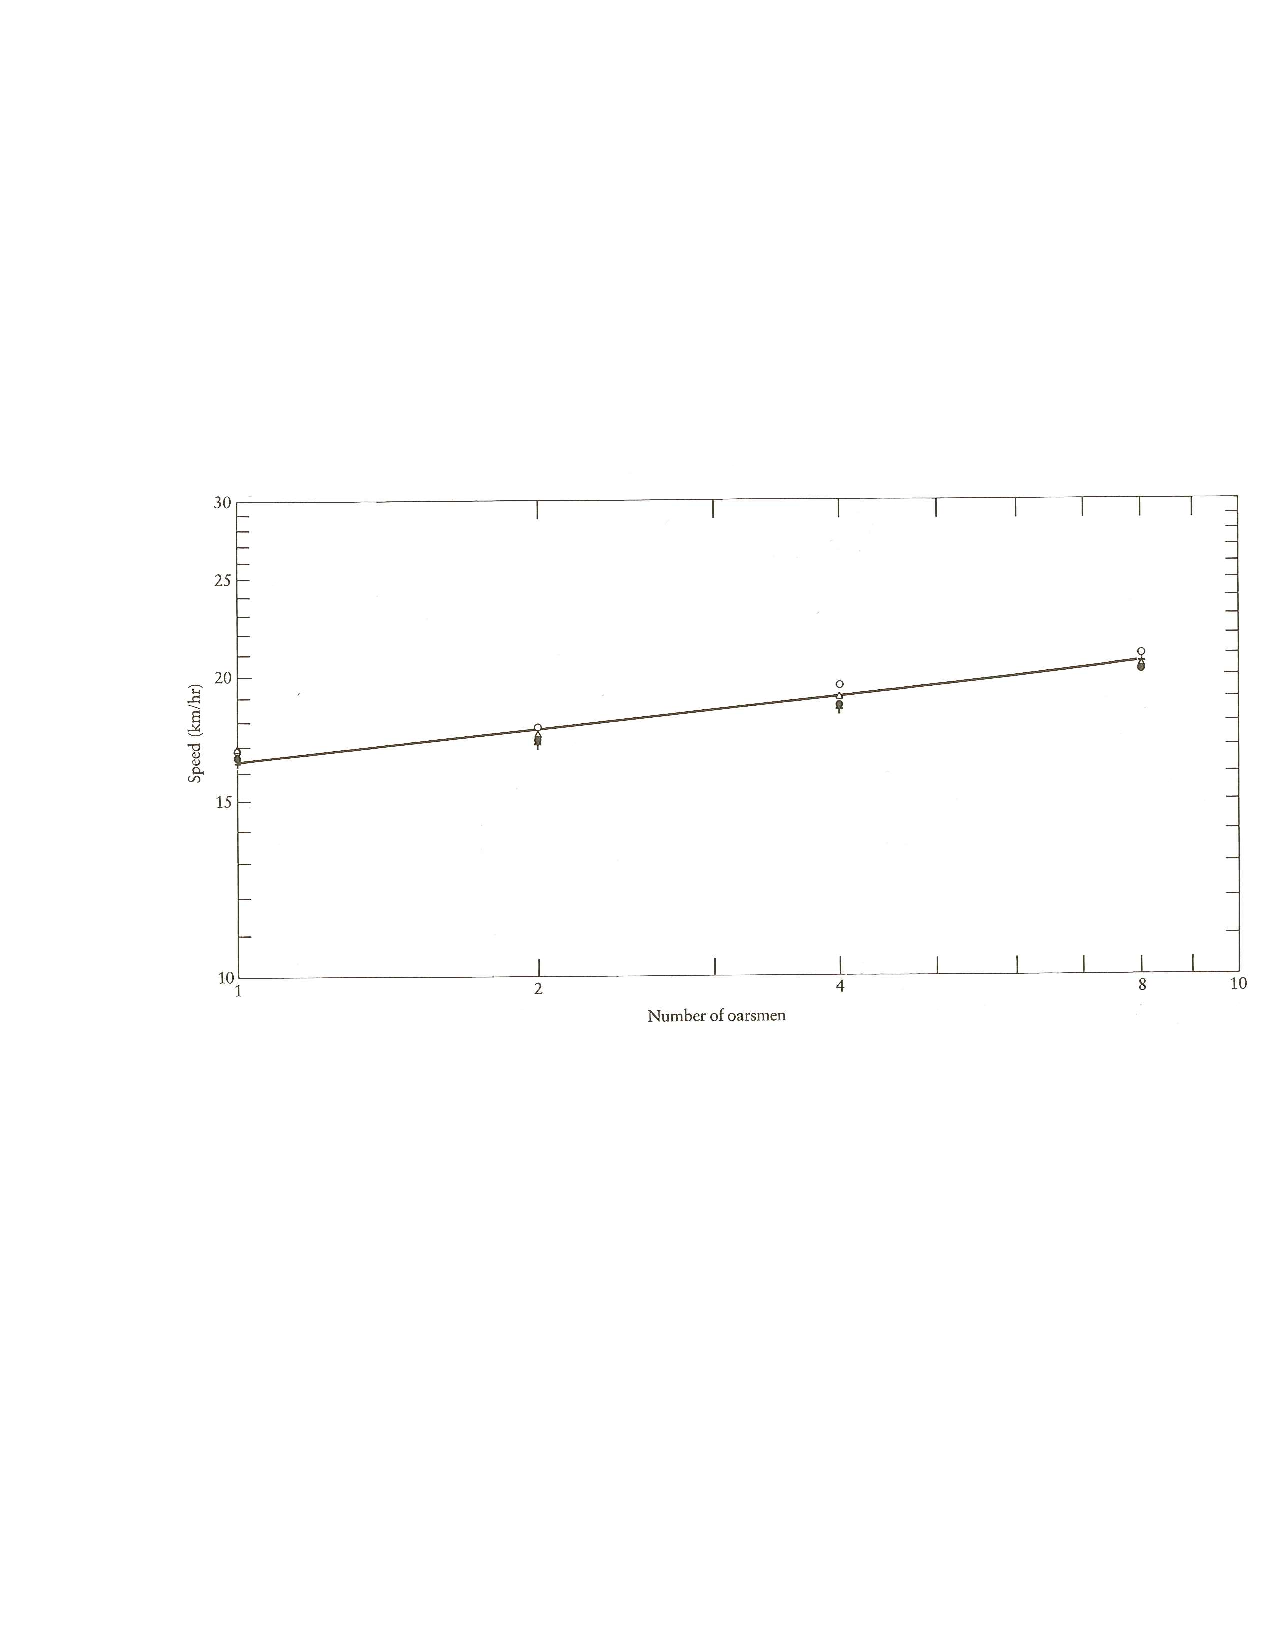
\includegraphics[width=0.8\textwidth]{mcmahon1983a_p47rowing.pdf}

  
   \solutionstart

   %% solution goes here

   \solutionend

  
\item
  Finish the calculation for the platypus on a pendulum problem
  so show that a simple pendulum's period $\tau$ is indeed proportional to
  $\sqrt{\ell / g}$.

  Basic plan from lectures: Create a matrix $\textmatrix{A}$
  where $ij$th entry is the power of dimension $i$ in the $j$th
  variable, and solve by row reduction to find basis null vectors.

  In lectures, we arrived at:
  \begin{equation}
  \textmatrix{A}\vec{x}
  =
  \mymatrix{cccc}{
    1 & 0 & 1 & 0 \\
    0 & 1 &  0 & 0 \\
    0 & 0 & -2 & 1 \\
  }
  \colvec{ x_{1} \\ x_{2} \\ x_{3} \\ x_{4} }
  = 
  \colvec{ 0 \\ 0 \\ 0}
  \end{equation}

  You only have to take a few steps from here.

  %% fall 2017: start 35
  %% fall 2016: start 56:14, end 1:12:08 
  %% fall 2015: start 25:05, end 46:20
  %%   \videohelp{TX-QmpPbWgE}{3374}{4328}{56:14}{1:12:08}{15:54}
  %%  From Season 10. Will update.

  From Lecture 3:
  the \wordwikilink{https://www.youtube.com/watch?v=_lPfMiLLinI}{Buckingham $\pi$ theorem} (20 minutes).
  
  
   \solutionstart

   %% solution goes here

   \solutionend

\item

  Show that the maximum speed of animals $V_{\textnormal{max}}$
  is proportional to their length $L$~\cite{meyer-vernet2015a}.
  Here are five dimensionful parameters:
  \begin{itemize}
  \item 
    $V_{\textnormal{max}}$, maximum speed.
  \item 
    $\ell$, animal length.
  \item 
    $\rho$, organismal density.
  \item 
    $\sigma$, maximum applied force per unit area of tissue.
  \item 
    $b$, maximum metabolic rate per unit mass
    ($b$ has the dimensions of power per unit mass).
  \end{itemize}
  
  And here are the three dimensions: $L$, $M$, and $T$.

  Use a back-of-the-envelope calculation to
  express $V_{\textnormal{max}} / \ell$ in terms
  of $\rho$, $\sigma$, and $b$.

  Note: It's argued in~\cite{meyer-vernet2015a}
  that these latter three parameters vary
  little across all organisms (we're mostly
  thinking about running organisms here),
  and so finding $V_{\textnormal{max}} / \ell$
  as a function of them indicates
  that $V_{\textnormal{max}} / \ell$ is also roughly constant.

  
   \solutionstart

   %% solution goes here

   \solutionend

\item
  Use the Buckingham $\pi$ theorem to reproduce G. I. Taylor's
  finding the energy of an atom bomb $E$ is related to
  the density of air $\rho$ and the radius of the blast wave $R$
  at time $t$:
  \begin{equation}
  E
  = 
  \mbox{constant} \times
  \rho R^5 / t^2.
  \end{equation}

  In constructing the matrix, order parameters as $E$, $\rho$, $R$, and $t$
  and dimensions as $L$, $T$, and $M$.

  
   \solutionstart

   %% solution goes here

   \solutionend

\item
  Use the Buckingham $\pi$ theorem to derive Kepler's third law,
  which states that the square of the orbital period of a planet
  is proportional to the cube of its semi-major axis.

  Let's shed some enlightenment and assume circular orbits.

  Parameters:
  \begin{itemize}
  \item
    Planet's mass $m$;
  \item
    Sun's mass $M_{\textnormal{sun}}$;
  \item
    Orbital period $\tau$;
  \item
    Orbital radius $r$;
  \item
    Graviational constant $G$.
  \end{itemize}

  \begin{enumerate}
  \item
    What are the dimensions of these five quantities?
  \item
    You will find that there are two dimensionless parameters
    using the Buckingham $\pi$ theorem, and that you can
    choose one to be $\pi_{2} = m/M_{\textnormal{sun}}$.
    Find the other dimensionless parameter, $\pi_{1}$.
  \item
    Now argue that $\tau^{2} \propto r^{3}$.
  \item
    For our solar system's nine (9) planets (yes, Pluto is on the team here), plot
    $\tau^{2}$ versus $r^{3}$, and using basic linear regression
    report on how well Kepler's third law holds up.
  \end{enumerate}
  
  
   \solutionstart

   %% solution goes here

   \solutionend
  

  
\end{enumerate}
